\documentclass{article}
\usepackage{amsmath, amssymb, amsthm}


\usepackage{graphicx}
\usepackage{tikz}

\usepackage{array}
\usepackage{xepersian}
\settextfont{XB Niloofar}

\newtheorem{theorem}{قضیه}
\newtheorem{lemma}{لم}

\begin{document}
	
	\title{کد پروفر و یکتایی آن برای درخت‌ها}
	\author{محمد حسین کاظمینی-محمد جواد عبدالهی}
	\date{1403/12/06}
	\maketitle
	
	\section{تعریف کد پروفر}
	\textbf{کد پروفر} یک دنباله عددی است که به هر درخت برچسب‌دار با $n$ راس نسبت داده می‌شود و یک نمایش فشرده از درخت ارائه می‌دهد. این کد، تناظر یک به یک بین درخت‌های برچسب‌دار و دنباله‌هایی به طول $n-2$ برقرار می‌کند.
	
	\section{الگوریتم تولید کد پروفر از درخت}
	برای تولید کد پروفر یک درخت با $n$ رأس:
	\begin{enumerate}
		\item کوچکترین برگ (راسی که درجه آن ۱ است) را پیدا کنید.
		\item همسایه آن را در دنباله پروفر ثبت کنید.
		\item برگ را از درخت حذف کنید.
		\item این کار را تا زمانی که فقط دو رأس باقی بماند، تکرار کنید.
	\end{enumerate}
	
	\subsection{مثال:}
	درخت زیر را در نظر بگیرید:
	
	\begin{center}
		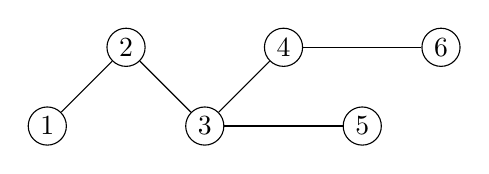
\begin{tikzpicture}[scale=1, every node/.style={circle, draw, inner sep=2pt}]
			\node (1) at (0,0) {1};
			\node (2) at (1,1) {2};
			\node (3) at (2,0) {3};
			\node (4) at (3,1) {4};
			\node (5) at (4,0) {5};
			\node (6) at (5,1) {6};
			
			\draw (1) -- (2);
			\draw (2) -- (3);
			\draw (3) -- (4);
			\draw (3) -- (5);
			\draw (4) -- (6);
		\end{tikzpicture}
	\end{center}
	
	فرآیند تولید کد پروفر به این صورت است:
	
	\begin{center}
		\begin{tabular}{|c|c|c|}
			\hline
			مرحله & برگ حذف شده & کد پروفر در این مرحله \\
			\hline
			1 & 1 (متصل به 2) & 2 \\
			2 & 2 (متصل به 3) & 3 \\
			3 & 5 (متصل به 3) & 3 \\
			4 & 3 (متصل به 4) & 4 \\
			\hline
		\end{tabular}
	\end{center}
	
	بنابراین، کد پروفر این درخت برابر است با:
	\[
	(2,3,3,4)
	\]
	
	\section{الگوریتم بازسازی درخت از روی کد پروفر}
	برای بازسازی درخت از روی کد پروفر:
	\begin{enumerate}
		\item درجه هر رأس را محاسبه کنید.
		\item کوچکترین رأسی که درجه آن ۱ است پیدا کرده و به اولین مقدار دنباله متصل کنید.
		\item درجه رأس متصل‌شده را کاهش دهید، برگ را حذف کرده و ادامه دهید.
		\item این کار را تا زمانی که دو رأس باقی بمانند انجام دهید و در نهایت آن‌ها را به هم متصل کنید.
	\end{enumerate}
	
	\subsection{مثال:}
	با استفاده از کد پروفر $(2,3,3,4)$، درخت را بازسازی می‌کنیم:
	
	\begin{center}
		\begin{tabular}{|c|c|c|}
			\hline
			مرحله & اتصال برقرار شده & کد پروفر باقی‌مانده \\
			\hline
			1 & 1 به 2 & (3,3,4) \\
			2 & 2 به 3 & (3,4) \\
			3 & 5 به 3 & (4) \\
			4 & 3 به 4 & () \\
			\hline
		\end{tabular}
	\end{center}
	
	در نتیجه درخت اصلی بازسازی شد. شکل نهایی درخت:
	
	\begin{center}
		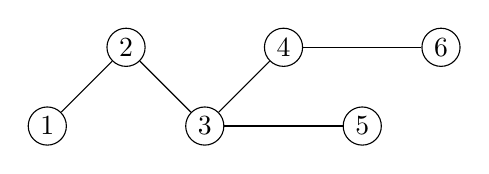
\begin{tikzpicture}[scale=1, every node/.style={circle, draw, inner sep=2pt}]
			\node (1) at (0,0) {1};
			\node (2) at (1,1) {2};
			\node (3) at (2,0) {3};
			\node (4) at (3,1) {4};
			\node (5) at (4,0) {5};
			\node (6) at (5,1) {6};
			
			\draw (1) -- (2);
			\draw (2) -- (3);
			\draw (3) -- (4);
			\draw (3) -- (5);
			\draw (4) -- (6);
		\end{tikzpicture}
	\end{center}
	
	\section{اثبات یکتایی}
	\begin{theorem}
		هر درخت دارای یک کد پروفر یکتاست.
	\end{theorem}
	\begin{proof}
		فرآیند کدگذاری همواره کوچکترین برگ را حذف کرده و تنها همسایه آن را در کد ثبت می‌کند. چون کوچکترین برگ همیشه به طور یکتا مشخص می‌شود، دو درخت مختلف نمی‌توانند کد پروفر یکسانی داشته باشند.
	\end{proof}
	
	\begin{theorem}
		هر کد پروفر به یک درخت یکتا منجر می‌شود.
	\end{theorem}
	\begin{proof}
		در فرآیند بازسازی، همیشه کوچکترین رأس با درجه ۱ به اولین مقدار دنباله متصل می‌شود. این فرآیند، در هر مرحله به طور یکتا مشخص شده و در نهایت یک درخت یکتا را نتیجه می‌دهد.
	\end{proof}
	
	\section{نتیجه‌گیری}
	کد پروفر نه‌تنها نمایش فشرده‌ای از درخت ارائه می‌دهد، بلکه می‌توان تعداد درخت‌های برچسب‌دار را نیز از آن نتیجه گرفت. تعداد درخت‌های ممکن با $n$ رأس برابر است با:
	\[
	n^{n-2}
	\]
	که معادل تعداد دنباله‌های پروفر یکتا است.
\end{document}
